\documentclass[12pt]{article}
\usepackage[margin=1.2in]{geometry}
\usepackage{graphicx}
\usepackage{amsmath}
\usepackage{physics}
\usepackage{tabto}
\usepackage{float}
\usepackage{amssymb}
\usepackage{pgfplots}
\usepackage{verbatim}
\usepackage{tcolorbox}
\usepackage{listings}
\usepackage{color}
\lstset{
    basicstyle=\ttfamily,
    showstringspaces=false,
    numbers=left,
    upquote=true,
    captionpos=b,
    abovecaptionskip=12pt,
    language=Python,
    breaklines=true,
    frame=single,
    framerule=2pt}
\renewcommand{\lstlistingname}{Appendix}
\pgfplotsset{compat=1.16}

\title{CP Activity 1: Plotting and Basic Data Analysis}
\author{\textbf{PHY2004W \hspace{8cm} KDSMIL001}}
\date{\textbf{17 Feb 2020}}

\begin{document}

    \begin{titlepage}
        \maketitle
        \tableofcontents
    \end{titlepage}

    \section{Introduction}
    This Computational Activity was created in order to reintroduce us to Python and to 
    give us a first look at Python modules such as numpy, scipy, and matplotlib. To perform 
    the tasks set for us by the activity we used a laptop which had Python 3.7 installed, 
    as well as the numpy, scipy, and matplotlib modules. 

    \section{Process}
    The first task set to us (CP1a) was to use numpy and scipy to calculate the mean value 
    and the variance of a set of data points given to us in the document Activity1Data.txt. 
    We expected to see the same results for each method of computing the values.
    Below is the code used to compute those values [Figure 5] as well as the results from 
    each method [Figure 1]. 

    \begin{figure}[H]
        \begin{center}
           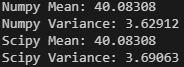
\includegraphics[scale=1]{CP1a results.png}
           \caption{CP1a Results}
           \label{Figure 1}
        \end{center}
    \end{figure}
    
    \noindent
    As can be seen in Figure 2, we saw a difference of about 0.06 between the values of 
    variance computed by numpy and scipy. After looking through the documentation of each 
    module we found that the var() function in the numpy module uses a biased formula to 
    find the variance, whereas the stats.describe() function from scipy uses an unbiased 
    formula to calculate variance. Note that if we had used the var() function from scipy, 
    we would have observed the same biased result as with the numpy var() function.
    \newline
    \newline
    The next part of the activity (CP1b) was an introduction to the module matplotlib, which 
    is used to produce publication quality plots. We were given a set of points with error 
    bounds for each and were asked to reproduce (exactly!) a plot provided to us. Below 
    is the code we used to produce the plot [Figure 6] as well as the plot itself [Figure 2]. 
    The final question of the activity asked us to plot the line of best fit for this plot, 
    which we have included in Figure 2.

    \begin{figure}[H]
        \begin{center}
           \input{CP1b plot.pgf}
           \caption{CP1b Plot}
           \label{Figure 2}
        \end{center}
    \end{figure}
    
    \noindent
    The third part of the activity (CP1c) was to write a program that would calculate $m$ 
    and $c$, as well as the uncertainties for both, from a set of data provided in the 
    document LinearNoErrors.txt. The code for this section can be found in Figure 7 \& 8 
    and the results are below [Figure 3]. The formulas used to find these values were 
    provided in the activity sheet. 
    
    \begin{figure}[H]
        \begin{center}
           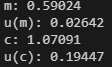
\includegraphics[scale=1]{CP1c results.png}
           \caption{CP1c Results}
           \label{Figure 3}
        \end{center}
    \end{figure}

    \newpage
    \noindent
    The final part of the activity (CP1d) was split into three parts. Firstly we were asked to 
    write another program to calculate the mean and variance of the original set of data, 
    ACtivity1Data.txt, using the given equations for each rather than relying on the 
    modules to do all the work. We decided to calculate both a biased and unbiased variance 
    in order to compare them to the values obtained in CP1a. What we saw was exactly what 
    we expected; the numpy variance was exactly what we obtained using the biased variance 
    formula, and the scipy variance was exactly what we had obtained using the unbiased 
    variance formula. These results can be seen below [Figure 4] and the code for this 
    program can be found in Figure 9. Do note that all values obtained from these 
    programs have been rounded to 5 decimal places.

    \begin{figure}[H]
        \begin{center}
           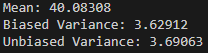
\includegraphics[scale=1]{CP1d part 1 results.png}
           \caption{CP1d Part 1 Results}
           \label{Figure 4}
        \end{center}
    \end{figure}
    
    \noindent
    Secondly, we were asked to comment on the measurement of x. The data provided to us was 
    an array of readings of x. What we did to the readings, calculating the mean and the 
    variance, provided us with measurement for x, namely $40.08 \pm 3.69$ if we use the 
    biased variance, which we should use as this is only a sample of the data, not the 
    entire population. This variance acts as the uncertainty of our measurement. In other 
    words, the variance is our confidence interval as it shows the interval around our 
    measurement that the actual value could lie it, given the readings that we have to consider.
    \newline
    \newline
    The final part of the activity was to plot the line of best fit for the data we used in 
    CP1b, which can be seen in Figure 2.
    \newline
    \newline
    The code for all of these questions can be found in the Appendix on the next page.
    

    \newpage
    \section{Appendix}

    \begin{figure}[H]
        \begin{center}
            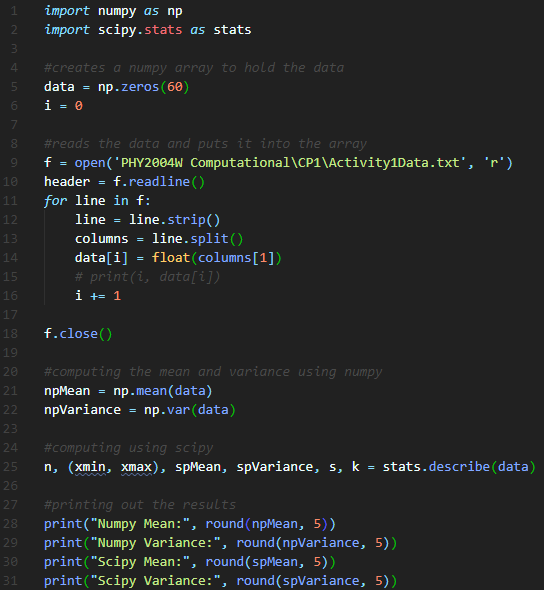
\includegraphics[scale=0.7]{CP1a code.png}
            \caption{CP1a Code}
            \label{Appendix 1}
        \end{center}
    \end{figure}

    \begin{figure}[H]
        \begin{center}
           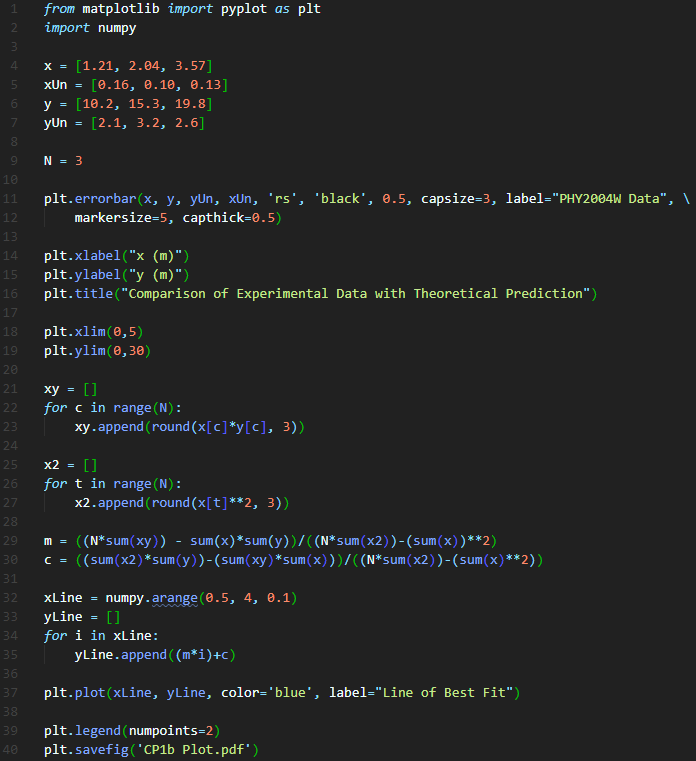
\includegraphics[scale=0.7]{CP1b code.png}
           \caption{CP1b Code}
           \label{Appendix 2}
        \end{center}
    \end{figure}

    \begin{figure}[H]
        \begin{center}
           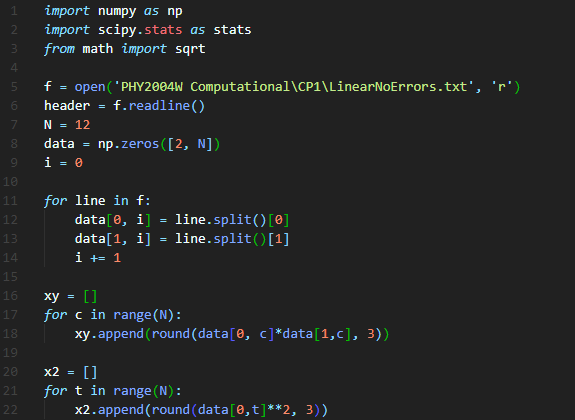
\includegraphics[scale=0.7]{CP1c code 1.png}
           \caption{CP1c Code 1}
           \label{Appendix 3}
        \end{center}
    \end{figure}
    
    \begin{figure}[H]
        \begin{center}
           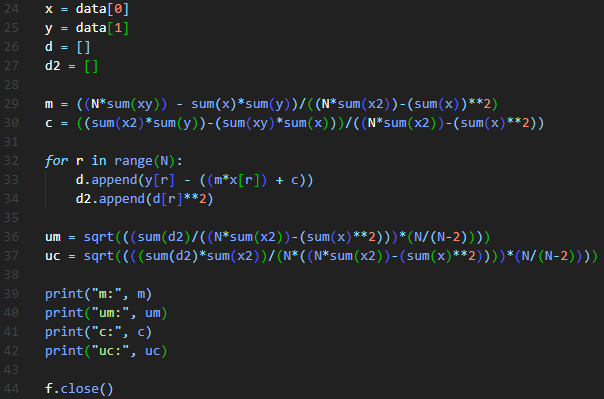
\includegraphics[scale=0.7]{CP1c code 2.png}
           \caption{CP1c Code 2}
           \label{Appendix 4}
        \end{center}
    \end{figure}
    
    \begin{figure}[H]
        \begin{center}
           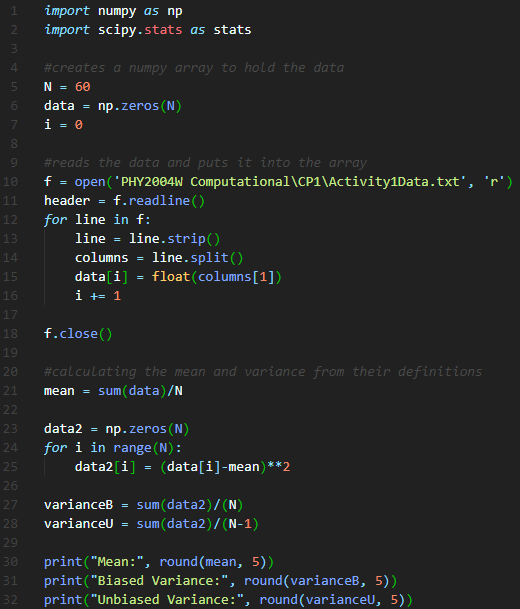
\includegraphics[scale=0.7]{CP1d part 1 code.png}
           \caption{CP1d Part 1 Code}
           \label{Appendix 5}
        \end{center}
    \end{figure}
    
    

\end{document}